\documentclass{article}

\usepackage[english]{babel}
\usepackage[utf8]{inputenc}
\usepackage{amsmath,amssymb}
\usepackage{parskip}
\usepackage{graphicx}

% Margins
\usepackage[top=2.5cm, left=3cm, right=3cm, bottom=4.0cm]{geometry}
% Colour table cells
\usepackage[table]{xcolor}

% Get larger line spacing in table
\newcommand{\tablespace}{\\[1.25mm]}
\newcommand\Tstrut{\rule{0pt}{2.6ex}}         % = `top' strut
\newcommand\tstrut{\rule{0pt}{2.0ex}}         % = `top' strut
\newcommand\Bstrut{\rule[-0.9ex]{0pt}{0pt}}   % = `bottom' strut

%%%%%%%%%%%%%%%%%
%     Title     %
%%%%%%%%%%%%%%%%%
\title{MLF HW1}
\author{\textbf{Junyi ZHONG} \\ MOSIG-M2-AIW\\  junyi.zhong@etu.univ-grenoble-alpes.fr}
\date{October 10, 2020}

\begin{document}
\maketitle

%%%%%%%%%%%%%%%%%
%   Problem 1   %
%%%%%%%%%%%%%%%%%
\section{Part 1: An analysis of the perceptron algorithm (10 Pts)}
The perceptron algorithm is one of the first supervised models proposed by Rosenblatt, 1957 for binary classification. The training step of the algorithm consists in finding the parameters of a linear function defined by


$\begin{aligned} h_{w}: \mathbb{R}^{d} & \rightarrow \mathbb{R} \\ \mathbf{x} & \mapsto\langle w, \mathbf{x}\rangle \end{aligned}$

using a training set $S=\left(\left(\mathbf{x}_{i}, y_{i}\right)\right)_{i=1}^{m}$ of size m where, ⟨., .⟩ denotes the dot product and the classes verify $\forall i \in\{1, \ldots, m\}, y_{i} \in\{-1,+1\}$ The training of the model is generally done on-line as it is shown in algorithm 1.

% Example of how to add figure (can be used for jpeg, png, pdf, eps etc)
\begin{figure}[h!]
    \centering
    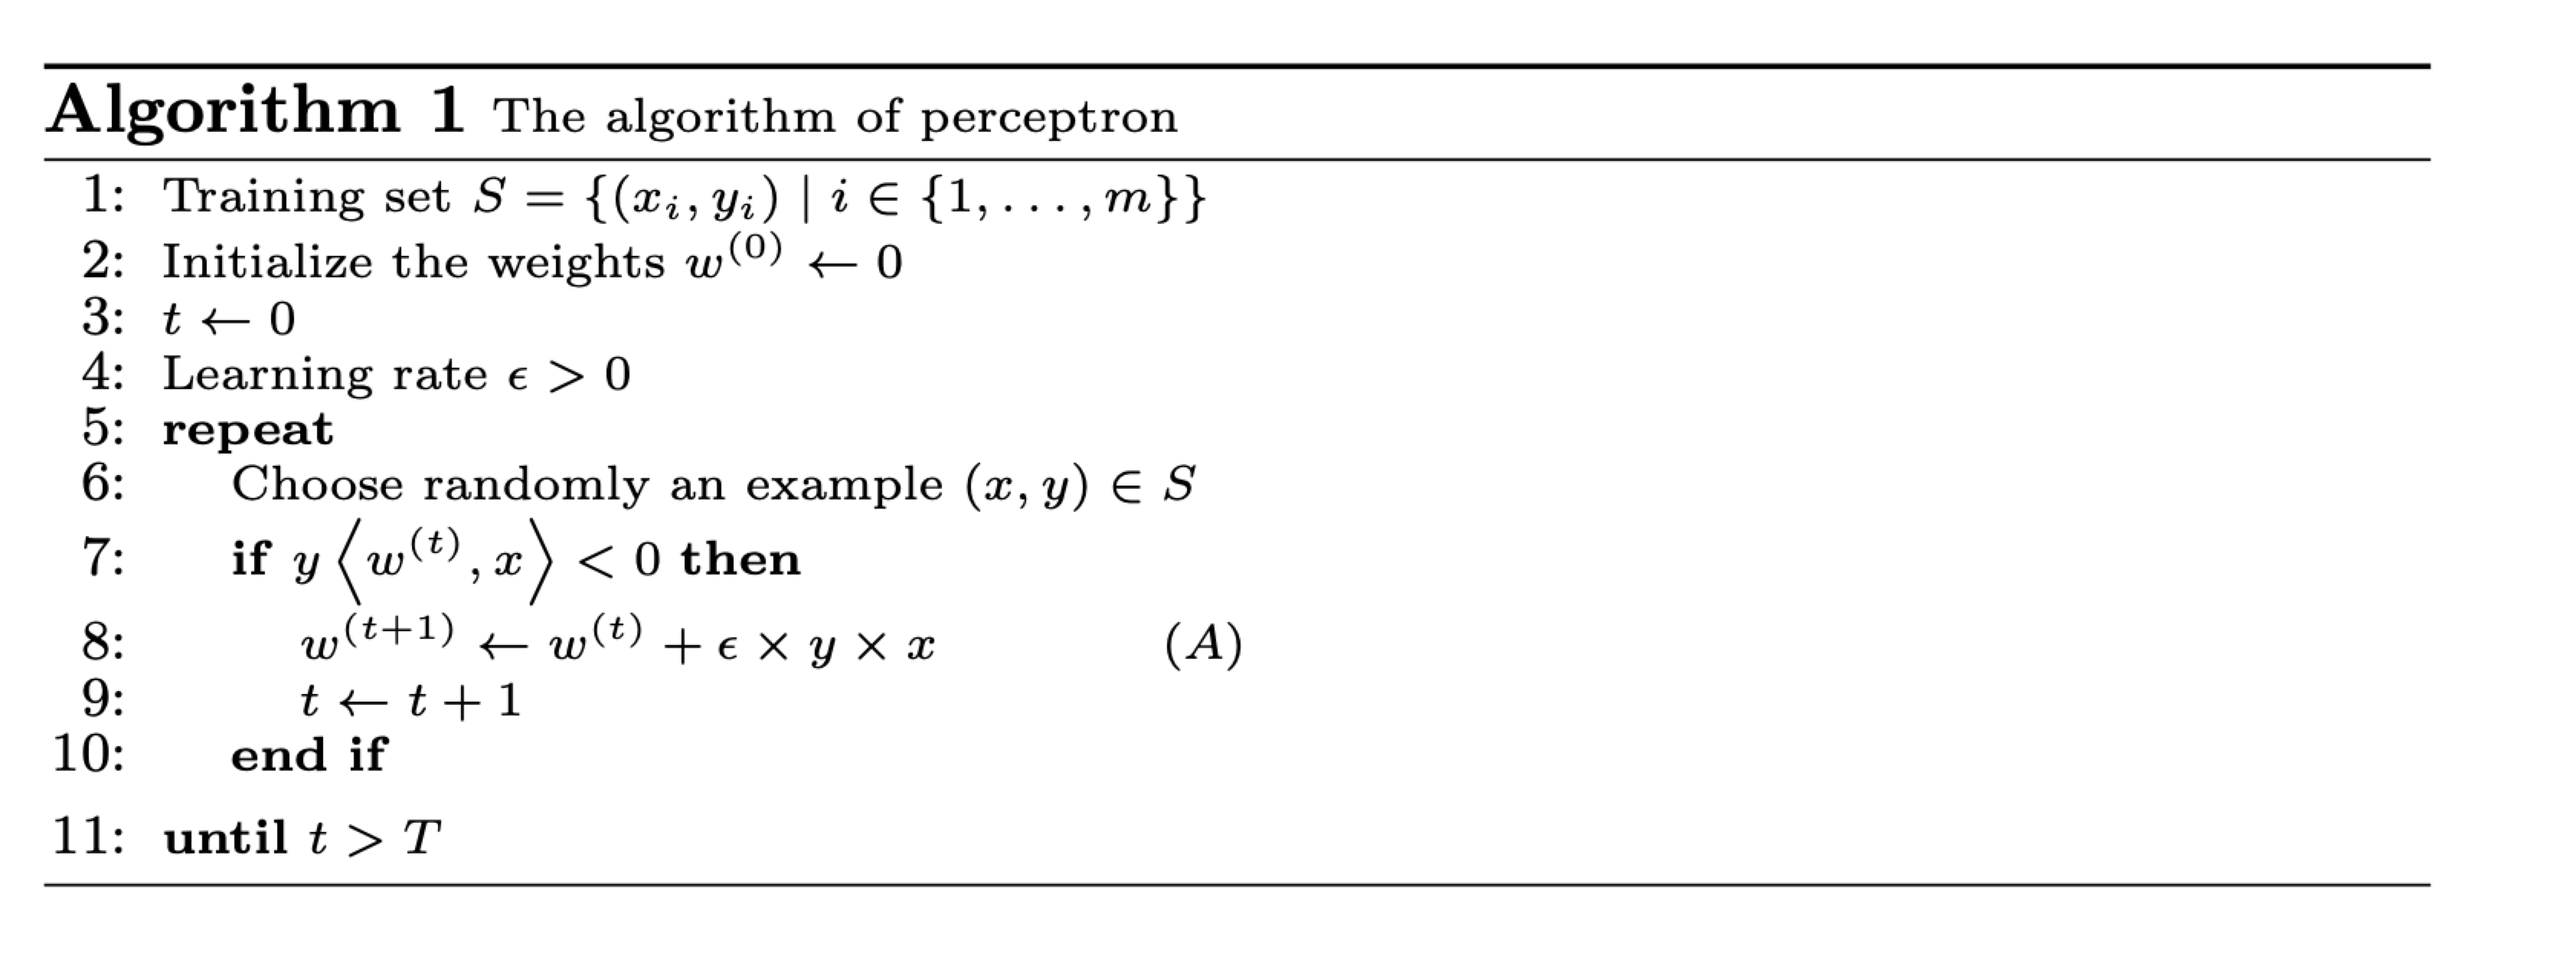
\includegraphics[scale=0.13]{perceptron.png}
    \caption{The algorithm of perceptron}
    \label{fig:universe}
\end{figure}
% Ex 1.1
 \subsection{\textbf{Explain the algorithm.}}
Answer:
\newline
\newline
\textbf{(What)}  The perceptron is an online algorithm which is used for supervised learning model to train binary linear classifiers. 

The perceptron consists of 4 parts.
\begin{enumerate}
\item 	Input values or One input layer
\item 	Weights and Bias
\item 	Net sum
\item 	Activation Function
\end{enumerate}

\textbf{(How)} The implementation follows the widely used online learning scheme where training examples are randomly chosen one at a time and the model's weight vector is updated based on the prediction error made by the current classifier. Consider the form of the linear classifier as $f(\mathbf{x})=\langle\mathbf{x}, \overline{\boldsymbol{w}}\rangle+w_{0}$, where $\mathbf{x} \in \mathbb{R}^{d}$ , $\overline{\boldsymbol{w}} \in \mathbb{R}^{d},$ and $w_{0} \in \mathbb{R}$  For each sample i in training set S,perform calculating the output and updating the weights to keep adjusting classification effect.

% EX 1.2
 \subsection{\textbf{How is called the update rule (eq. (A)), and what does it do?}}
Answer:
\newline
\newline
-1.2.1 Update rule is for each training sample x(i),use gradient descent,to calculate the output value and update the weights to get a hyperplane to perfectly classify data points.

-1.2.2 The idea is keep minimizing errors. The value for updating the weights at each increment is calculated by the learning rule:
$\forall t \geq 1, \boldsymbol{w}^{(t)} \leftarrow \boldsymbol{w}^{(t-1)}-\eta \nabla_{\boldsymbol{w}^{(t-1)}} \hat{\mathcal{L}}\left(\boldsymbol{w}^{(t-1)}\right)$

though learning rule to adjust hyperplane classification effect, until no misclassification data points, reach convergence. 
% (Usually define the MSE (the mean squared error) as the loss function of the perceptron. Then update the weighs using gradient descent and back-propagation (just like any other neural network).
%  EX 1.3
 \subsection{\textbf{Consider the following classification problem in a two dimensional space.Suppose that the chosen example is x3, what will be the new weight vector using the update rule of the perceptron if $\epsilon=1$? Draw the weight vector by reproducing the figure in your sheet.\\}}

Answer:
\newline 
% Example of how to add figure (can be used for jpeg, png, pdf, eps etc)
\begin{figure}[h!]
    \centering
    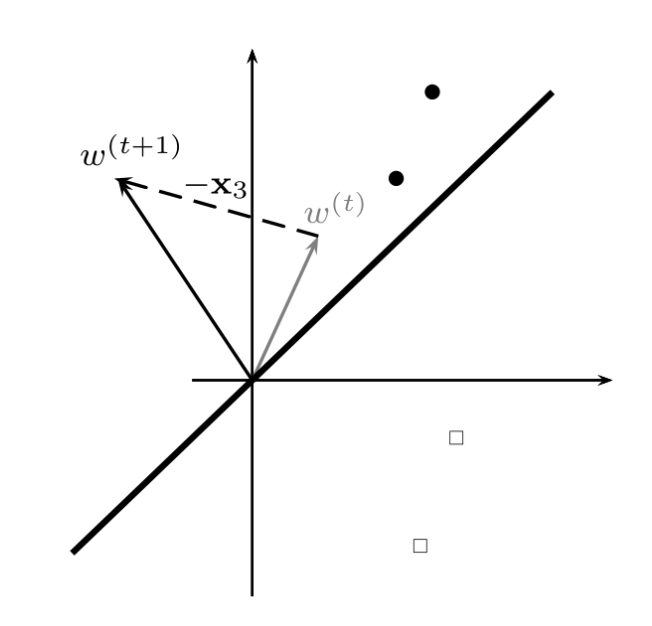
\includegraphics[scale=0.5]{figure-2-d.png}
    \caption{}
    \label{}
\end{figure}
%  EX 1.4
\subsection{\textbf{We are now interested to demonstrate the convergence of the algorithm in a finite number of iterations and in the case where there exists a weight vector w∗ such that $\forall\left(\mathbf{x}_{i}, y_{i}\right) \in S ; y_{i} \times\left\langle w^{*}, \mathbf{x}_{i}\right\rangle>0$ What is the meaning of the condition $y \times\left\langle w^{*}, \mathbf{x}\right\rangle>0 ?$}}

Answer:
\newline 
$y \times\left\langle w^{*}, \mathbf{x}\right\rangle>0 $ means predicate positive, there is no miss-classified data point for all the samples.
\newline



% EX 1.5
 \subsection{\textbf{We suppose that there exists w∗ such that$\forall\left(\mathbf{x}_{i}, y_{i}\right) \in S ; y_{i} \times\left\langle w^{*}, \mathbf{x}_{i}\right\rangle>0$ 
and we define $\rho=\min _{i \in\{1, \ldots, m\}}\left(y_{i}\left\langle\frac{w^{*}}{|| w^{*}||}, \mathbf{x}_{i}\right\rangle\right)$ What does $\rho$ represent? Explain why it is a strictly positive real value?}}
Answer:
\newline
$\rho$ of the hyperplane w*, which is the distance from this hyperplane to the closet data point. The essence of minimization is to make the classification hyperplane as correct as possible. 
 \newline
 Because $y \times\left\langle w^{*}, \mathbf{x}\right\rangle>0 $},  output is correct classification which requests  $\rho > 0$,,  thus  $\rho$,is a absolute positive value.

% EX 1.6
\subsection{\textbf{We suppose that all the examples in the training set are within a hypersphere of radius $R$ (i.e. $\forall \mathbf{x}_{i} \in S,\left\|\mathbf{x}_{i}\right\| \leq R$ ). Further, we initialise the weight vector to be the null vector (i.e. $\left.w^{(0)}=0\right)$ as well as the learning rate $\epsilon=1 .$ Show that after $t$ updates, the norme of the current weight vector satisfies :
$$
\left\|w^{(t)}\right\|^{2} \leq t \times R^{2}
$$
hint : You can consider $\left\|w^{(t)}\right\|^{2}$ as $\left\|w^{(t)}-w^{(0)}\right\|^{2}$}}
Answer:\newline
As the normal vector hyperplane $w^{*}$ perfectly separates the examples of the two classes, i.e. $\forall\left(\mathbf{x}_{i}, y_{i}\right) \in S ; y_{i} \times\left\langle w^{*}, \mathbf{x}_{i}\right\rangle>0$ it means that learning rate $ \rho> 0. $ Moreover, after t updates with the perceptron learning rule $\forall(\mathbf{x}, y),$ if $y\left(\langle\overline{\boldsymbol{w}}, \mathbf{x}\rangle+w_{0}$  and considering the previous initialization, we consider 
\newline
$\left\|w^{(t)}\right\|^{2}=\left\|w^{(t)}-w^{(0)}\right\|^{2}=\left\|w^{(t-1)}+y^{(t)} \times \mathbf{x}^{(t)}-w^{(0)}\right\|^{2}$
\newline\newline
where $\left(\mathrm{x}^{(t)}, y^{(t)}\right)$is the $\ell^{m e}$ example wrong class of the sequence after $t-1$ updates the weight vector. According to the triangular inequality and the condition 
$\forall i \in\{1, \ldots, m\},\left\|\mathbf{x}_{i}\right\| \leqslant R$
\newline we have
\newline 
$\left\|\boldsymbol{w}^{(t)}\right\|^{2} \leqslant\left\|\boldsymbol{w}^{(t-1)}\right\|^{2}+\left\|\mathbf{x}^{(t)}\right\|^{2} \leqslant\left\|\boldsymbol{w}^{(t-1)}\right\|^{2}+R^{2}$
\newline 
\newline
With the same reasoning,we also have
\newline
\newline
$\left\|w^{(t-1)}\right\|^{2} \leqslant\left\|w^{(t-2)}\right\|^{2}+R^{2}, \ldots$ 
and $\left\|w^{(1)}\right\|^{2} \leqslant R^{2},$  
\newline
so
\newline 
$\left\|w^{(t)}\right\|^{2} \leqslant t \times R^{2}$

or in another way the same idea,
because of $\epsilon=1,  y_{i}^{2}=1, \quad 2 \epsilon x_{i} y_{i} w^{(t-1)}<0$
so 

$\begin{aligned}\left\|\hat{w}_{t}\right\|^{2} &=\left\|\hat{w}_{t-1}+\epsilon y_{i} \hat{x}_{i}\right\|^{2} \\ &=\left\|\hat{w}_{t-1}\right\|^{2}+2 \epsilon y_{i} \hat{w}_{t-1} \cdot \hat{x}_{i}+\epsilon^{2} y_{i}^{2}\left\|\hat{x}_{i}\right\|^{2} \\ &=\left\|\hat{w}_{t-1}\right\|^{2}+2 \epsilon y_{i} \hat{w}_{t-1} \cdot \hat{x}_{i}+\epsilon^{2}\left\|\hat{x}_{i}\right\|^{2} \\ & \leq\left\|\hat{w}_{t-1}\right\|^{2}+\epsilon^{2}\left\|\hat{x}_{i}\right\|^{2} \leq\left\|\hat{w}_{t-1}\right\|^{2}+\epsilon^{2} R^{2} \\ & \leq\left\|\hat{w}_{t-2}\right\|^{2}+2 \epsilon^{2} R^{2} \leq \cdots \leq t \epsilon^{2} R^{2} \end{aligned}$

% EX1.7
\subsection{\textbf{Using the the same condition than in the previous question, show that after $t$ updates of the weight vector we have
$$
\left\langle\frac{w^{*}}{\left\|w^{*}\right\|}, w^{(t)}\right\rangle \geq t \times \rho
$$}}
Answer:
\newline
% $\hat{w}_{o p t}$ is an optimal hyperplane, $\hat{w}_{o p t}=\frac{\left|w^{*}\right|}{\|w\|}$,
\newline
$\begin{aligned} w^{(t)} &=w^{(t-1)}+\epsilon y_{i} x_{i} \\ \frac{w^{*}}{\left\|w^{*}\right\|} \cdot w^{(t)} &=\left(w^{(t-1)}+\epsilon y_{i} x_{i}\right) \frac{w^{*}}{\left\|w^{*}\right\|} \\ &=w^{(t-1)} \cdot \frac{w^{*}}{\left\|w^{*}\right\|}+\epsilon y_{i} x_{i} \cdot \frac{w^{*}}{\left\|w^{*}\right\|} \end{aligned}$
\newline
because of,
\newline
$$
\rho \leq y_{i}\left(\frac{w^{*}}{\left\|w^{*}\right\|}, x_{i}\right)
$$
So,
$$
\begin{aligned}
\frac{w^{*}}{\left\|w^{*}\right\|} \cdot w^{(t)} & \geqslant w^{(t-1)} \cdot \frac{w^{*}}{\| w^{*} \mid}+\epsilon \rho \\
& \geqslant w^{(t-2)} \cdot \frac{w^{*}}{\left\|w^{*}\right\|}+2 p \\
&=\ldots \\
& \geqslant t \cdot \rho
\end{aligned}
$$
% $t \epsilon \rho \leq \hat{w}_{t} \hat{w}_{o p t} \leq\left\|\hat{w}_{t}\right\|\left\|\hat{w}_{o p t}\right\|=\left\|\hat{w}_{t}\right\| \leq \sqrt{t} \epsilon^{2} R^{2}$


%EX 1.8 
\subsection{\textbf{Deduce from equations (1) and (2) that the number of iterations $t$ is bounded by
$$
t \leq\left(\left(\frac{R}{\rho}\right)^{2}\right]
$$
where $\lfloor x\rfloor$ represents the floor function (This result is due to Novikoff, 1966)}}
Answer:
\newline

Combining the bounds in Eqs. 1 and 2 gives:\newline
$\begin{aligned} t ·\rho \leqslant\left(\frac{w^{*}}{\| w^{*}||} \cdot w^{(t)}\right) & \leqslant\left\|w^{(t)}\right\| \cdot\left\|\frac{w^{*}}{\left\|w^{*}\right\|}\right\| \\ & \leq\left\|w^{(t)}\right\| \leqslant R \cdot \sqrt{t} \end{aligned}$
\newline
$t^{2} \rho^{2} \leq\left\|\underline{\omega}{ }^{t+1}\right\|^{2}
\leq t R^{2}$ 
\newline
from which it follows that
$$
t \leq \frac{R^{2}}{\rho^{2}}
$$
t is the number of misclassified iterations,
% EX 1.9
\subsection{\textbf{Explain the previous result}}
Answer:
This is a proof of Novikoff's Theorem convergence,  this algorithrm is only for linearly separable case, we have a bound over the maximum number of updates t, then there is no instance of misclassification, model will be convergent.
\end{document}
